\chapter{Specifications}
This chapter tries to shed light on what was before this internship and why all the achieved work was
needed.

\section{Overall goal}
The principal purpose of this internship is to improve an algorithm already implemented and used to
minimize \textit{deterministic} $\omega$-automaton. The source code associated is the result of two papers:
\begin{itemize}
 \item \textbf{SAT-based Minimization of Deterministic $\omega$-Automata~\cite{15}} and
 \item \textbf{Mechanizing the Minimization of Deterministic Generalized Büchi Automata~\cite{14}}.
\end{itemize}

Those two papers written by \textit{Souheib baarir} and \textit{Alexandre Duret-Lutz} are themselves a
generalization of \textbf{Ehlers}' SAT-based procedure~\cite{17}. Note that the first paper~\cite{15} is an
extension of the second~\cite{14} which is restricted to generalized-Büchi acceptance.

\subsection{The existing minimization}

The existing minimization is based on this observation: since the reference automaton $R$ (the inputed one)
is complete and deterministic and the candidate automaton $C$ (the mininal one to find) is also complete
and deterministic, any word of $\Sigma^\omega$ has a unique run in $R$ and $C$. Verifying that both
automaton recognizes the same language can be done by ensuring that each word is accepted by $R$ iff it is
accepted by $C$. In practice, this is checked by ensuring that any cycle of the synchronous product
$C \otimes R$ corresponds to cycles that are either accepting in $C$ and $R$, or rejecting in both.\\

These previous work introduced a tool called \textsc{Synthetize}DTGBA$(R,n,m)$ that can read any
\textit{deterministic} $\omega$-automaton and synthetize (if it exists) an equivalent \textit{deterministic}
$\omega$-automaton with a given number of states and arbitrary acceptance condition. It works this way:
\begin{itemize}
 \item[-] inputs a complete DTGBA $R$, two target numbers of state ($n$) and arbitrary acceptance condition
          ($m$),
 \item[-] produces a DIMACS file~\cite{18} with all necessary clauses,
 \item[-] calls a SAT solver to solve this problem,
 \item[-] builds the resulting DTGBA $C$ if it exists.
\end{itemize}

\noindent Using this tool, two minimization algorithms have been implemented:
\begin{algorithm}[H]
 \caption{A naive algorithm that calls \textsc{Synthetize}DTGBA$(R,n,m)$ in a loop, with a decreasing
          number of states, and returns the last successfully built automaton.}
 \label{naive}
 \begin{algorithmic}[1]
  \Procedure{\textsc{ReduceStatesDTGBA}$(R,m=R$.nb\_acc\_sets()$)$}{}
   \BState \emph{repeat}:
   \State $n \gets R.nb\_states() $
   \State $C \gets \textsc{Synthetize}DTGBA(R,n-1,m) $
   \If {$C$ \textbf{does not exists}} \Return $R$\EndIf
   \State $R \gets C$
  \EndProcedure
 \end{algorithmic}
\end{algorithm}

\begin{algorithm}[H]
 \caption{This also calls \textsc{Synthetize}DTGBA$(R,n,m)$ in a loop, but attempting to find the minimum
          number of states using a binary search.}
 \label{dicho}
 \begin{algorithmic}[1]
  \Procedure{\textsc{DichotomyDTGBA}$(R,m=R$.nb\_acc\_sets()$)$}{}
   \State $max\_states \gets R.nb\_states()-1$
   \State $min\_states \gets 1$
   \State $S \gets null$
   \While{$min\_states \leq max\_states$}
    \State $target \gets \lfloor(max\_states + min\_states) / 2\rfloor$
    \State $C \gets \textsc{Synthetize}DTGBA(R,target,m)$
    \If {$C$ \textbf{does not exists}}
     \State $min\_states \gets target + 1$
    \Else
     \State $S \gets C$
     \State $max\_states \gets R.nb\_states()-1$
    \EndIf
   \EndWhile
   \State $R \gets S$
  \EndProcedure
 \end{algorithmic}
\end{algorithm}

\noindent Until this internship, Algorithm~\ref{naive} was used by default. There are no real reasons for
that except that the second algorithm was implemented later in a completely different context and has never
been benchmarked and compared to the first one.\\

\noindent \textbf{$\omega$-Automata minimization} can be seen in two ways:
\begin{itemize}
 \item \textbf{Reduction of the number of states:}
       This is typically the algorithm~\ref{naive} that keeps by default the same number of acceptance sets
       ($m$) and decreases $n$ at each \textsc{Synthetize}DTGBA$(R,n,m)$ call. The algorithm~\ref{dicho}
       has also the same perception. It knows the minimal automaton is between $1$ (obviously, a smaller
       one does not exists) and $n-1$ so instead of checking each number of states it performs a binary
       search with the will to be faster.
 \item \textbf{Rise of the accepting sets number:}
       This can be interpreted as the converse of a degeneralization: instead of augmenting the number
       of states to reduce the number of acceptance sets, we augment the number of acceptance sets in
       an attempt to reduce the number of states.
\end{itemize}

\noindent The figure below~\ref{fig:accsets} is a great example from the first paper~\cite{14} that shows how
smaller an automaton can become if the acceptance sets number is increased. Note that $|\mathcal{F}|$ here
is $m$ (the number of accepting sets).
\begin{figure}[H]
 \centering
 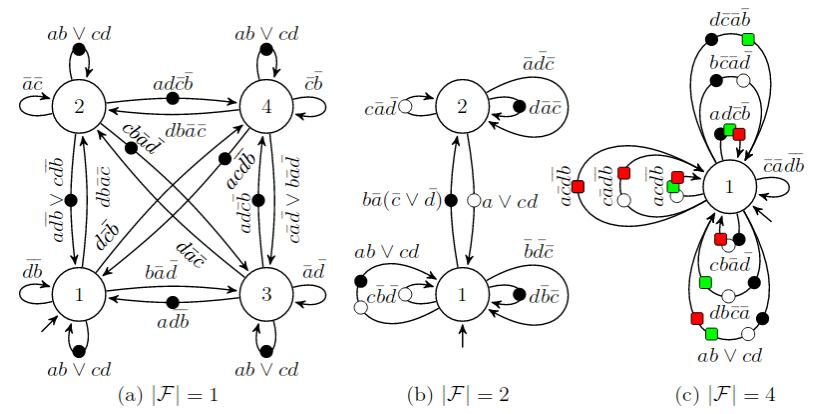
\includegraphics[scale=0.5]{img/accsets_reduction.png}
 \caption{Examples of minimal DTGBA recognizing $(GFa \land GFb) \lor (GFc \land GFd)$}
 \label{fig:accsets}
\end{figure}

Finding the smallest $m$ such that no smaller equivalent DTGBA with a larger $m$ can be found is
still an opened problem.

\subsection{Tool chain}
The figure~\ref{fig:tool_chain} (from the FORTE'14 paper~\cite{14}) gives an overview of the processing
chains that can be used to turn an LTL formula~\cite{13} into minimal DBA, DTBA or DTGBA.
The blue area at the top describes:
\begin{lstlisting}[language=bash,caption={bash command-line to translate a formula using ltl2tgba}]
  ltl2tgba -D -x sat-minimize
\end{lstlisting}

\noindent while the purple area at the bottom corresponds to:
\begin{lstlisting}[language=bash,caption={bash command-line to translate a formula using dstar2tgba}]
  dstar2tgba -D -x stat-minimize
\end{lstlisting}

\begin{figure}[H]
 \centering
 \tikzstyle{dstep}=[align=center,minimum height=3em]
\tikzstyle{pstep}=[draw,dstep,drop shadow,fill=white]
\tikzstyle{iostep}=[dstep,rounded corners=1mm]
\tikzstyle{instep}=[iostep,fill=yellow!20]
\tikzstyle{outstep}=[iostep,fill=green!20]
\tikzstyle{errstep}=[iostep,fill=red!20]

\begin{tikzpicture}[shorten >=1pt,>=stealth',semithick,node distance=5.5mm]
%\tikzset{callout/.style={ellipse callout, callout pointer arc=30,
%  callout absolute pointer={#1},fill=blue!30,draw}}
%\tikzstyle{

\node[pstep] (trans) {translate\\to TGBA};
\node[pstep,right=of trans.0,xshift=-2mm] (wdba) {attempt\\WDBA\\minim.};
\draw[->] (trans) -- (wdba);
\node[pstep,right=of wdba.0] (simp) {simplify\\TGBA};
\draw[->] (wdba) -- node[above]{fail} (simp);
\node[instep,below=of trans,yshift=-2mm] (ltl1) {LTL\\formula};
\draw[->] (ltl1) -- (trans);

\node[pstep,right=of simp,yshift=8mm,xshift=1mm] (degen) {degen\\to TBA};
\draw[->] (simp) -- ($(simp.east)+(2mm,0mm)$) |- node[above left,align=right,at end]{nondet. or\\$|\CF|>m=1$} (degen);
\coordinate[pstep,right=of degen,yshift=-8mm,xshift=-1mm] (isdet);
%\coordinate[pstep,right=of degen,yshift=-2em] (isdet2);
\draw[->] (simp) -- ($(simp.east)+(2mm,0mm)$) -- node[below right,at start]{else} (isdet);
\coordinate  (degen2) at ($(degen.east)+(2mm,0mm)$);
\draw[->] (degen) -- (degen2) -- ($(simp.east -| degen2)$);
\node[pstep,right=of degen,xshift=2.5em] (tbadet) {attempt\\ powerset\\to DTBA};
\draw[->] (isdet) |- node[at end,above left]{nondet.} (tbadet);
\coordinate  (tbadet2) at ($(tbadet.east)+(2mm,0mm)$);
\node[errstep,right=of tbadet.0,xshift=2mm,yshift=2mm] (nottcong) {not in\\$\mathsf{TCONG}$};
\draw[->] (tbadet) -- node[at end,above left,align=center]{fail} ($(nottcong.180 |- tbadet)$);
\coordinate (turn) at ($(nottcong.-130 |- simp.0)$);
\draw[->] (isdet) -- node[below right,at start]{det.} (turn);
\draw[->] (tbadet2) -- node[right,pos=.6]{success} ($(tbadet2 |- turn)$);
\node[pstep,below=of tbadet.-125,yshift=-3mm] (dtbasat) {DTBA SAT\\minimization};
\node[pstep,below=of dtbasat,yshift=5mm] (dtgbasat) {DTGBA SAT\\minimization};
\draw[->] (turn) |- node[above left]{$m=1$} (dtbasat);
\draw[->] (turn) |- node[above left]{$m>1$} (dtgbasat);
\node[outstep,left=of dtgbasat] (mindtgba) {minimal\\DTGBA};
\node[outstep] at ($(mindtgba |- dtbasat)$) (mindtba) {minimal\\DTBA};
\node[outstep,left=of mindtba,xshift=5mm] (wdbaok) {minimal\\WDBA};
\draw[->] (wdba) |- coordinate(c1) node[above right]{success} (wdbaok);

\draw[->] (dtgbasat) -- (mindtgba);
\draw[->] (dtbasat) -- (mindtba);
\node[pstep,below=of ltl1,yshift=-2mm,xshift=1mm] (ltl2dstar) {\texttt{ltl2dstar}\\(DRA)};
\draw[->] (ltl1) -- ($(ltl1 |- ltl2dstar.90)$);
\node[pstep,right=of ltl2dstar] (dra2dba) {attempt\\conversion\\to DBA};
\draw[->] (ltl2dstar) -- (dra2dba);
\node[pstep,right=of dra2dba,xshift=3em] (wdba2) {attempt\\WDBA\\minim.};
\node[pstep,right=of wdba2,xshift=2em] (simp2) {simplify as\\DBA or DTBA};
\draw[->] (dra2dba) -- node[at start,below right]{success} (wdba2);
\draw[->] (wdba2) -- node[at start,below right]{fail} (simp2);
\coordinate (turn2) at ($(turn |- simp2)$);
\draw[->] (simp2) -- (turn2);
\draw[] (turn2) -- (turn);
\node[errstep] (notrec) at ($(ltl1 -| dra2dba)$) {not a\\ recurrence};
\draw[->] (dra2dba) -- node[right]{fail} (notrec);
\draw[->] (wdba2.160) -| node[below right,sloped]{success} (wdbaok);

\begin{scope}[on background layer]
\coordinate (pt1) at ($(tbadet.north east)+(3mm,2mm)$);
\coordinate (pt2) at ($(mindtba.north east)+(3mm,0mm)$);
\coordinate (pt3) at ($(mindtgba.south east)+(0mm,-1mm)$);
\coordinate[xshift=1mm,yshift=1mm] (turn3) at (turn);
\path[pattern color=blue!30,pattern=north west lines] ($(trans.west |- pt1)$) |- (pt2) |- (pt3) -| (turn3) -| (pt1) --  cycle;
\node[below right] at ($(trans.west |- pt1)$) {\texttt{ltl2tgba}};


\coordinate[yshift=1mm,xshift=1mm] (pt4) at ($(pt2 -| turn3)$);
\coordinate[yshift=-3mm,xshift=-1mm] (pt5) at ($(dra2dba.south west)$);
\coordinate[yshift=1mm,xshift=-1mm] (pt6) at ($(dra2dba.north west)$);
\path[pattern color=blue!30!red!30,pattern=north east lines] (pt5) -| (pt4)  -- ($(pt2) + (1mm,1mm)$) |- (pt6) -- cycle;
\node[above left,yshift=-1mm] at ($(pt5 -| pt4)$) {\texttt{dstar2tgba}};
\end{scope}

%\node[fill=yellow,draw,ellipse callout,thin,inner sep=0.5pt,callout pointer arc=30,,yshift=6mm,callout absolute pointer={(c1)}] at (c1) {\footnotesize 1};

\end{tikzpicture}

 \caption{Two tool chain used to convert an LTL formula}
 \label{fig:tool_chain}
\end{figure}

\noindent As the SAT-based minimization only takes DTBA or DTGBA, the input automaton undergoes some
transformations. In each tool, a Weak-DBA minimization is attempted. If that succeed, a minimal weak DBA
is outputed (looking for transition-based or generalized acceptance will not reduce it further). For
further details, please read the FORTE'14 paper~\cite{14}.

\subsection{The limits}
Consider again the default algorithm (~\ref{naive}).
At each iteration, this algorithm re-encodes the research of a smaller automaton from scratch. Iterations
after iterations (from $n$ to $n-1$, $n-1$ to $n-2$, etc.) the clauses encoded are almost the same.
Therefore, it is a shame that nothing is retained, learned at each iteration. This is where incremental sat
solving comes in mind.\\

Incremental solving is one of the recent directions in SAT solver research. This is
based on an observation that in many applications of SAT solvers, the problems being solved consist of
several calls to SAT solver on a sequence of SAT problem. Typically, the problems in the sequence share a
large common part, making them highly interrelated. This is exactly our case! The purpose of incremental
SAT solving is to recycle the work done in solving a previous problem in the sequence to solve the
subsequent problems.\\

In order to use an incremental approach with SAT solver, it is no more possible to use DIMACS file
~\cite{18}. Therefore, Spot needs to be linked to a SAT solving library. Let's remember that until now
Spot requires a SAT solver to be installed on the same machine and provides a way to set it (through
SPOT\_SATSOLVER environment variable). obviously, being linked to a SAT solver and make calls to its
functions will be more efficient than making Input/Output operations and executing another binary.\\

The memory consumption is also another problem. The larger the automaton is, the more variables there are.
With some automata, the memory usage could grow over 150 Go which is uncommon for most users. The figure
~\ref{fig:over_memory} helps to see memory usage peaks during a benchmark realized the end of September
2016.\\

\begin{figure}[h]
 \centering
 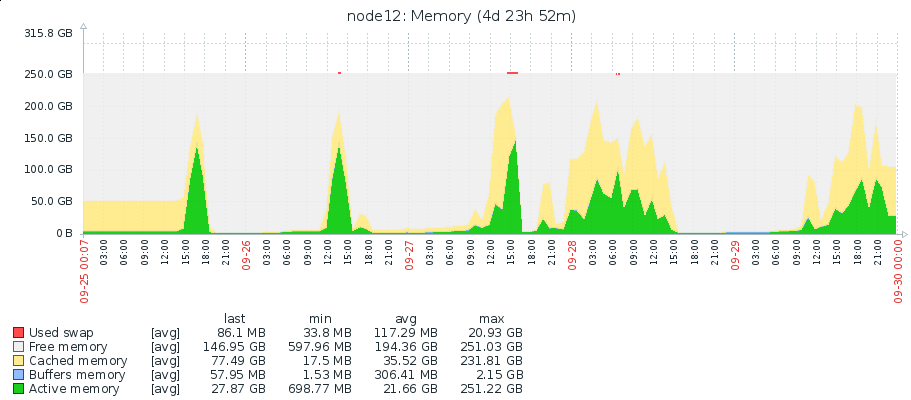
\includegraphics[scale=0.5]{img/over_memory.png}
 \caption{A graph showing memory usage during a benchmark realized at the beginning of the internship}
 \label{fig:over_memory}
\end{figure}

\section{Detailed explanation of the results to be obtained}
As said before, the purpose of this internship is to improve the current SAT-based minimization technique.
This minimization is wanted to be more fast and less greedy in memory consumption.
If you look at the tool chain section above, this internship intervenes in the two SAT minimization
rectangles (for $m=1$ and $m > 1$).\\

The idea of testing an incremental approach for SAT-based minimization has already been raised by the Spot
team. \textit{Alexandre Duret-Lutz} had a clear idea of how to do it and I had been assigned the task of
testing this idea. The objective being to improve it as mush as possible, the internship is not limited
to that. It is a line of approach as many others and the results to obtain can lead to new reflections.\\

\begin{algorithm}[H]
 \caption{An incremental approach that does the same traditional encoding once and then tries to exclude
          one more state at each iteration of a loop. The encoding is never restarted.}
 \label{incr1}
 \begin{algorithmic}[1]
  \Procedure{\textsc{ReduceStatesDTGBA}$(R,m=R$.nb\_acc\_sets()$)$}{}
   \State $n \gets R.nb\_states() $
   \State $C \gets \textsc{Synthetize}DTGBA(R,n-1,m) $
   \If {$C$ \textbf{does not exists}} \Return $R$\EndIf
   \BState \emph{repeat}:
   \State add clauses to exclude one more state
   \State $C \gets$ Try to solve the new problem and build the new automaton
   \If {$C$ \textbf{does not exists}} \Return $R$\EndIf
   \State $R \gets C$
  \EndProcedure
 \end{algorithmic}
\end{algorithm}

To do so, Spot needs to be linked to a SAT solving library. The really first task is to know which. I had
to find the more suitable SAT solver that fills those requirements:
\begin{itemize}
 \item It must have a compatible licence with Spot's one. Spot is under a GNU General Public Licence 3.
 \item It has to be maintained.
 \item It must be simple to integrate with Spot. Simple means here that the code shall be modified as little
       as possible so that a future update to a newer version of that solver will be simple to achieve.
 \item It must be easy to use as library.
 \item Of course, it has to be efficient. Therefore, a look to SAT solvers international competitions as
       well as a custom benchmark is a fundamental need.
\end{itemize}

\noindent Regarding the memory consumption, the purpose is to identify the most memory-hungry parts of the
source code and come up with solutions.\\

The results to be obtained can not be more precise than that. There is no precise figure estimating the
speed to reach for a particular formula or the exact memory consumption to reduce, etc.\\

It is an internship that is part of a research work. By definition, the results are often unpredictable.